\documentclass{article}
\PassOptionsToPackage{numbers, compress}{natbib}
\usepackage[]{nips_2018}  % Options: preprint, final, nonatbib
% General packages:
\usepackage[T1]{fontenc}     % Encoding
\usepackage[english]{babel}  % Naming of figures and such
\usepackage{hyperref}        % Clickable references
\usepackage{microtype}       % Nice typography
\usepackage{etoolbox}        % Tools

% Page layout:
\usepackage{setspace}        % Line spacing
\usepackage{ragged2e}        % Better line endings
\usepackage[
    parfill
    ]{parskip}               % Newlines instead of indentation
\usepackage[
    hang,
    bottom
    ]{footmisc}              % Configure footnotes

% Utility:
\usepackage[table]{xcolor}   % Colours
\usepackage[
    separate-uncertainty=true,
    per-mode=symbol
    ]{siunitx}               % Display units
\usepackage{enumitem}        % Better enumeration
\usepackage{xifthen}         % If statements
\usepackage{lipsum}          % Dummy text
\usepackage{blindtext}       % More dummy text
\usepackage{listings}        % Listings
\usepackage{xparse}          % Better arguments for \newcommand

% Figures:
\usepackage{pgfplots}        % Plots
\pgfplotsset{compat=newest}
\usepackage{tikz}            % TikZ figures
\usepackage{float}           % Control floating of figures
\usepackage{multirow}        % Cells spanning multiple rows
\usepackage{graphicx}        % Graphics
\usepackage{caption}         % Subfigures and captions
\usepackage{subcaption}      % Subfigures and captions
\usepackage{booktabs}        % Nice looking tables
\usepackage{tabularx}        % Extended functionality for tables

% Math:
\usepackage{amsmath}         % Math
\usepackage{amssymb}         % Math symbols
\usepackage{mathtools}       % Math tools
\usepackage{amsthm}          % Theorems
\usepackage{thmtools}        % More math theorems
\usepackage{bbm}             % Bold math symbols
\usepackage{cancel}          % Cancel equations

% Math:
\usepackage{amsmath}         % Math
\usepackage{amssymb}         % Math symbols
\usepackage{mathtools}       % Math tools
\usepackage{amsthm}          % Theorems
\usepackage{thmtools}        % More math theorems
\usepackage{bm}              % Bold math symbols
\usepackage{bbm}             % Blackboard math symbols
\usepackage{cancel}          % Cancel equations

\usepackage{todonotes}

% This package should be loaded last.
\usepackage[
    noabbrev,
    capitalize,
    nameinlink]{cleveref}    % Automatic referencing
    
% \ifempty command:
\newcommand{\ifempty}[3]{\ifthenelse{\equal{#1}{}}{#2}{#3}}

% Style footnotes.
\setlength{\skip\footins}{\baselineskip}
\renewcommand{\footnotelayout}{\setstretch{1.5}}
\setlength{\footnotemargin}{1em}

% Typewriter font:
\renewcommand*{\ttdefault}{pcr}  % Courier
\newcommand{\code}[1]{\texttt{#1}}

% Define some colours.
\definecolor{darkblue} {rgb} {0.0 , 0.0 , 0.65}
\definecolor{darkred}  {rgb} {0.80, 0.0 , 0.0 }
\definecolor{darkgreen}{rgb} {0.0 , 0.50, 0.0 }
\definecolor{gray75}   {gray}{0.75}

% Define shortcuts for colours.
\newcommand{\red}[1]{{\color{red} #1}}
\newcommand{\blue}[1]{{\color{blue} #1}}
\newcommand{\green}[1]{{\color{green} #1}}
\newcommand{\darkred}[1]{{\color{darkred} #1}}
\newcommand{\darkblue}[1]{{\color{darkblue} #1}}
\newcommand{\darkgreen}[1]{{\color{darkgreen} #1}}
\newcommand{\magenta}[1]{{\color{magenta} #1}}
\newcommand{\grey}[1]{{\color{gray} #1}}

% Load TikZ libraries.
\usetikzlibrary{
    calc,
    positioning,
    fit,
    tikzmark,
    arrows.meta,
    shapes,
    decorations.pathreplacing
}
% Graphical models:
\tikzset{
    line/.style = {
        thick,
        ->,
        > = {
            Triangle[length=2.0mm, width=2.0mm]
        }
    },
    arrow/.style = {
        line
    },
    % Invisible node:
    hidden node/.style = {
        circle,
        minimum size = 1cm,
        draw = white,
        thick
    },
    % Latent variable:
    latent node/.style = {
        hidden node,
        draw = black,
    },
    % Latent variable:
    factor node/.style = {
        hidden node,
        rectangle,
        draw = black,
    },
    % Observed variable:
    observed node/.style = {
        latent node,
        fill = gray!15
    },
    % Plate:
    plate/.style = {
        draw,
        label={[anchor=north west]south west:#1},
        rounded corners=2pt,
        shape=rectangle,
        inner sep=10pt,
        thick
    }
}
% Set the default float placement correctly.
\floatplacement{figure}{htbp}
\floatplacement{table}{htbp}

% Set spacing between figures and text.
\setlength{\textfloatsep}{30pt plus 1.0pt minus 2.0pt}
\setlength{\floatsep}{30pt plus 1.0pt minus 2.0pt}
\setlength{\intextsep}{30pt plus 1.0pt minus 2.0pt}

% Define outline tools.
\newcommand{\outline}[1]{
    \parbox{\linewidth}{
        \singlespacing
        \color{darkgreen}
        #1
    }\vspace{\parsep}
}
\newlist{outlinelist}{enumerate}{1}
\setlist[outlinelist]{
    label=\arabic*.,
    noitemsep,
    topsep=0pt,
    parsep=0pt,
    partopsep=0pt
}
\newcommand{\note}[1]{{\color{darkred}#1}}

% Left-justified text in tabularx environment:
\newcolumntype{L}{>{\RaggedRight\arraybackslash}X}

% Hyperlink setup
\hypersetup{
    colorlinks,
    citecolor = black,
    filecolor = black,
    linkcolor = black,
    urlcolor  = black
}

% Scale TikZ pictures up.
\tikzset{
    every picture/.append style = {
        xscale = 2,
        yscale = 2
    }
}
% Define \charfusion. From https://tex.stackexchange.com/a/52673.
\makeatletter
\def\moverlay{\mathpalette\mov@rlay}
\def\mov@rlay#1#2{\leavevmode\vtop{%
   \baselineskip\z@skip \lineskiplimit-\maxdimen
   \ialign{\hfil$\m@th#1##$\hfil\cr#2\crcr}}}
    \newcommand{\charfusion}[3][\mathord]{
        #1{\ifx#1\mathop\vphantom{#2}\fi
        \mathpalette\mov@rlay{#2\cr#3}}
        \ifx#1\mathop\expandafter\displaylimits\fi
    }
\makeatother

% Bold characters:
\renewcommand{\vec}[1]{\boldsymbol{#1}}
\newcommand{\vecu}[1]{\hat{\vec{#1}}}
\newcommand{\mat}[1]{\vec{#1}}

% Letters commonly used in blackboard bold font:
\newcommand{\C}{\mathbb{C}}
\newcommand{\E}{\mathbb{E}}
\newcommand{\K}{\mathbb{K}}
\newcommand{\N}{\mathbb{N}}
\renewcommand{\P}{\mathbb{P}}
\newcommand{\Q}{\mathbb{Q}}
\newcommand{\R}{\mathbb{R}}
\newcommand{\eR}{\overline{\mathbb{R}}}
\newcommand{\V}{\mathbb{V}}
\newcommand{\Z}{\mathbb{Z}}

% Letters commonly used in calligraphic font:
\newcommand{\A}{\mathcal{A}}
\newcommand{\B}{\mathcal{B}}
\newcommand{\Cc}{\mathcal{C}}
\newcommand{\D}{\mathcal{D}}
\newcommand{\Ec}{\mathcal{E}}
\newcommand{\F}{\mathcal{F}}
\newcommand{\G}{\mathcal{G}}
\renewcommand{\H}{\mathcal{H}}
\newcommand{\J}{\mathcal{J}}
\newcommand{\Jrat}{\mathcal{J}_{\text{rat}}}
\renewcommand{\L}{\mathcal{L}}
\newcommand{\Li}{\mathcal{L}{}^1}
\newcommand{\eLi}{\overline{\mathcal{L}}{}^1}
\newcommand{\m}{\text{m}}
\newcommand{\M}{\mathcal{M}}
\newcommand{\eM}{\overline{\mathcal{M}}}
\newcommand{\Nc}{\mathcal{N}}
\renewcommand{\O}{\mathcal{O}}
\newcommand{\Rc}{\mathcal{R}}
\renewcommand{\S}{\mathcal{S}}
\newcommand{\Tc}{\mathcal{T}}
\newcommand{\U}{\mathcal{U}}
\newcommand{\Vc}{\mathcal{V}}
\newcommand{\W}{\mathcal{W}}
\newcommand{\X}{\mathcal{X}}
\newcommand{\Y}{\mathcal{Y}}
\newcommand{\Zc}{\mathcal{Z}}

% Letters commonly used in sans serif font:
\newcommand{\T}{\text{\textsf{T}}}
\renewcommand{\c}{\text{\textsf{c}}}

% Symbols:
\newcommand{\es}{\varnothing}
\newcommand{\e}{\varepsilon}
\newcommand{\sub}{\subseteq}
\renewcommand{\d}{\partial}
\renewcommand{\th}{\theta}
\newcommand{\Th}{\Theta}

% Convergence symbols:
\newcommand{\oto}[1]{\overset{#1}{\to}}
\newcommand{\uto}[1]{\underset{#1}{\to}}
\newcommand{\outo}[2]{\overset{#1}{\underset{#2}{\to}}}
\newcommand{\Lto}[1]{\oto{\L^{#1}}}

% Operators:
\DeclareMathOperator*{\argmax}{arg\,max\,}
\DeclareMathOperator*{\argmin}{arg\,min\,}
\let\max\relax\DeclareMathOperator*{\max}{max\,}
\let\min\relax\DeclareMathOperator*{\min}{min\,}
\let\sup\relax\DeclareMathOperator*{\sup}{sup\,}
\let\inf\relax\DeclareMathOperator*{\inf}{inf\,}
\let\limsup\relax\DeclareMathOperator*{\limsup}{lim\,sup\,}
\let\liminf\relax\DeclareMathOperator*{\liminf}{lim\,inf\,}
\newcommand{\card}{\#}
\newcommand{\cconv}{\circledast}
\newcommand{\chol}{\operatorname{chol}\,}
\newcommand{\ch}{\operatorname{ch}\,}
\newcommand{\cliques}{\operatorname{cliques}\,}
\newcommand{\cl}{\operatorname{cl}\,}
\newcommand{\col}{\operatorname{col}\,}
\newcommand{\comp}{\circ}
\newcommand{\contains}{\supseteq}
\newcommand{\conv}{\ast}
\newcommand{\cov}{\operatorname{cov}\,}
\newcommand{\diag}{\operatorname{diag}\,}
\renewcommand{\dim}{\operatorname{dim}\,}
\newcommand{\dotcup}{\charfusion[\mathbin]{\cup}{\cdot}}
\newcommand{\dotunion}{\charfusion[\mathop]{\bigcup}{\cdot}}
\newcommand{\had}{\circ}
\renewcommand{\Im}{\operatorname{Im}\,}
\newcommand{\ind}{\mathbbm{1}}
\newcommand{\intersection}{\bigcap}
\newcommand{\KL}{\operatorname{D}_{\text{KL}}}
\newcommand{\KOT}{\operatorname{KOT}\,}
\newcommand{\kron}{\otimes}
\newcommand{\MOT}{\operatorname{MOT}\,}
\newcommand{\push}{_\#}
\newcommand{\rank}{\operatorname{rank}\,}
\renewcommand{\Re}{\operatorname{Re}\,}
\newcommand{\row}{\operatorname{row}\,}
\newcommand{\schur}{\operatorname{Schur}\,}
\newcommand{\sign}{\operatorname{sign}\,}
\newcommand{\supp}{\operatorname{supp}\,}
\newcommand{\tr}{\operatorname{tr}\,}
\newcommand{\union}{\bigcup}
\newcommand{\vecspan}{\operatorname{span}\,}
\newcommand{\vol}{\operatorname{vol}\,}

% Probability distributions:
\newcommand{\Ber}{\operatorname{Ber}}
\newcommand{\Beta}{\operatorname{Beta}}
\newcommand{\Bin}{\operatorname{Bin}}
\newcommand{\Cat}{\operatorname{Cat}}
\newcommand{\Dir}{\operatorname{Dir}}
\newcommand{\Exp}{\operatorname{Exp}}
\newcommand{\Gam}{\operatorname{Gamma}}
\newcommand{\Geom}{\operatorname{Geom}}
\newcommand{\GP}{\mathcal{GP}}
\newcommand{\InvWishart}{\mathcal{W}^{-1}}
\newcommand{\LogNormal}{\log\mathcal{N}}
\newcommand{\Mult}{\operatorname{Mult}}
\newcommand{\NegBin}{\operatorname{NegBin}}
\newcommand{\Normal}{\mathcal{N}}
\newcommand{\Poisson}{\operatorname{Poisson}}
\newcommand{\Wishart}{\mathcal{W}}

% Probability commands:
\newcommand{\Var}{\V}
\newcommand{\Lik}{\L}

% Special math commands:
\newcommand{\cond}{\, | \,}                % Conditioning
\newcommand{\middlecond}{\, \middle| \,}   % Conditioning between a \left and \right
\newcommand{\divsep}{\,\|\,}               % Separator in divergences

\newcommand{\sd}[1]{\mathrm{d} #1}         % Straight 'd' in integral
\newcommand{\isd}[1]{\, \mathrm{d} #1}     % Straight 'd' in integral with spacing

\newcommand{\idf}{\text{\textsf{id}}}      % Identity function
\newcommand{\sce}{\text{\sc{e}}}           % Scientific notation
\newcommand{\vardot}{\,\cdot\,}            % Variable dot
\renewcommand{\ss}[1]{_\mathit{#1}}        % Subscripts without spacing

% Half refactangle
\newcommand{\halfrect}[2]{[\![#1,#2)\hspace{-1pt}\!)}
\newcommand{\Rint}{\text{(R)}\int}

% Paired delimiters:
\DeclarePairedDelimiter\parens{(}{)}           % Parentheses
\DeclarePairedDelimiter\sbrac{[}{]}            % Square brackets
\DeclarePairedDelimiter\cbrac{\{}{\}}          % Curly braces
\DeclarePairedDelimiter\set{\{}{\}}            % Set
\DeclarePairedDelimiter\lra{\langle}{\rangle}  % Angle brackets

% Shortcuts for angle brackets:
\newcommand{\la}{\langle}
\newcommand{\ra}{\rangle}
\newcommand{\lla}{\left\langle}
\newcommand{\rra}{\right\rangle}

% Other commands:
\newcommand{\resp}[1]{[#1]}                  % Respective statement
\newcommand{\bs}{\textbackslash}             % Blackslash in text
% Use \cref in a title.
\newcommand{\creftitle}[2]{\texorpdfstring{\cref{#2}}{#1 \ref{#2}}}
\newcommand{\mcheckthis}{{}^{[\checkmark]}}  % Checkmark in math
\newcommand{\checkthis}{$\mcheckthis$}       % Checkmark in text

% Compatibility with old commands:
\newcommand{\id}[1]{\sd{#1}}
\newcommand{\sargmax}[1]{\argmin_{#1}}
\newcommand{\sargmin}[1]{\argmax_{#1}}
\newcommand{\lrset}[1]{\set*{#1}}
\newcommand{\middleCond}{\middlecond}
\newcommand{\rel}[2]{($(#1) + (#2)$)}
\newcommand{\blackLinks}{}
\newcommand{\Ac}{\A}
% Define environments.
\newlength{\thmtopsep}\setlength{\thmtopsep}{\topsep + \parskip + .5\baselineskip}
\newlength{\thmbotsep}\setlength{\thmbotsep}{\topsep + .5\baselineskip}
\newtheoremstyle{theoremstyle}
    {\thmtopsep}{\thmbotsep}
    {}           % Body font
    {}           % Indent amount
    {\bfseries}  % Theorem head font
    {.}          % Punctuation after theorem head
    {.5em}       % Space after theorem head
    {}           % Theorem head spec
\theoremstyle{theoremstyle}

\newtheorem{assumption}{Assumption}[section]
\newtheorem{corollary}{Corollary}[section]
\newtheorem{definition}{Definition}[section]
\newtheorem{example}{Example}[section]
\newtheorem{fact}{Fact}[section]
\newtheorem{lemma}{Lemma}[section]
\newtheorem{model}{Model}[section]
\newtheorem{proposition}{Proposition}[section]
\newtheorem{remark}{Remark}[section]
\newtheorem{theorem}{Theorem}[section]

% Define environment QED markers.
\preto{\assumption}{\renewcommand\qedsymbol{$\blacktriangleleft$}\pushQED{\qed}}
\preto{\endassumption}{\popQED}
\preto{\corollary}{\renewcommand\qedsymbol{$\blacktriangleleft$}\pushQED{\qed}}
\preto{\endcorollary}{\popQED}
\preto{\definition}{\renewcommand\qedsymbol{$\blacktriangleleft$}\pushQED{\qed}}
\preto{\enddefinition}{\popQED}
\preto{\example}{\renewcommand\qedsymbol{$\blacktriangleleft$}\pushQED{\qed}}
\preto{\endexample}{\popQED}
\preto{\fact}{\renewcommand\qedsymbol{$\blacktriangleleft$}\pushQED{\qed}}
\preto{\endfact}{\popQED}
\preto{\lemma}{\renewcommand\qedsymbol{$\blacktriangleleft$}\pushQED{\qed}}
\preto{\endlemma}{\popQED}
\preto{\model}{\renewcommand\qedsymbol{$\blacktriangleleft$}\pushQED{\qed}}
\preto{\endmodel}{\popQED}
\preto{\proposition}{\renewcommand\qedsymbol{$\blacktriangleleft$}\pushQED{\qed}}
\preto{\endproposition}{\popQED}
\preto{\remark}{\renewcommand\qedsymbol{$\blacktriangleleft$}\pushQED{\qed}}
\preto{\endremark}{\popQED}
\preto{\theorem}{\renewcommand\qedsymbol{$\blacktriangleleft$}\pushQED{\qed}}
\preto{\endtheorem}{\popQED}

\newtheoremstyle{proofstyle}
    {\thmtopsep}{\thmbotsep}
    {}           % Body font
    {}           % Indent amount
    {\itshape}   % Theorem head font
    {.}          % Punctuation after theorem head
    {.5em}       % Space after theorem head
    {}           % Theorem head spec
\theoremstyle{proofstyle}
\let\proof\relax
\newtheorem*{proof}{Proof}
\AtEndEnvironment{proof}{\hfill{}Q.E.D.}

% Set referencing formats.
\crefname{assumption}{Assumption}{Assumptions}
\Crefname{assumption}{Assumption}{Assumptions}
\crefname{corollary}{Corollary}{Corollaries}
\Crefname{corollary}{Corollary}{Corollaries}
\crefname{definition}{Definition}{Definitions}
\Crefname{definition}{Definition}{Definitions}
\crefname{example}{Example}{Examples}
\Crefname{example}{Example}{Examples}
\crefname{fact}{Fact}{Facts}
\Crefname{fact}{Fact}{Facts}
\crefname{lemma}{Lemma}{Lemmas}
\Crefname{lemma}{Lemma}{Lemmas}
\crefname{model}{Model}{Models}
\Crefname{model}{Model}{Models}
\crefname{proposition}{Proposition}{Propositions}
\Crefname{proposition}{Proposition}{Propositions}
\crefname{remark}{Remark}{Remarks}
\Crefname{remark}{Remark}{Remarks}
\crefname{theorem}{Theorem}{Theorems}
\Crefname{theorem}{Theorem}{Theorems}

% Style enumerate:
\setenumerate{}
\setlist[enumerate]{label=(\arabic*)}
\setlist[itemize]{label=\textbullet}

% Referentiable list items in environments
\newlist{asslist}{enumerate}{1}
\setlist[asslist]{ref=\theassumption.(\arabic*), label=(\arabic*)}
\crefname{asslisti}{Assumption}{Assumptions}
\Crefname{asslisti}{Assumption}{Assumptions}
\newlist{corlist}{enumerate}{1}
\setlist[corlist]{ref=\thecorollary.(\arabic*), label=(\arabic*)}
\crefname{corlisti}{Corollary}{Corollaries}
\Crefname{corlisti}{Corollary}{Corollaries}
\newlist{deflist}{enumerate}{1}
\setlist[deflist]{ref=\thedefinition.(\arabic*), label=(\arabic*)}
\crefname{deflisti}{Definition}{Definitions}
\Crefname{deflisti}{Definition}{Definitions}
\newlist{exlist}{enumerate}{1}
\setlist[exlist]{ref=\thexample.(\arabic*), label=(\arabic*)}
\crefname{exlisti}{Example}{Examples}
\Crefname{exlisti}{Example}{Examples}
\newlist{factlist}{enumerate}{1}
\setlist[factlist]{ref=\thefact.(\arabic*), label=(\arabic*)}
\crefname{factlisti}{Fact}{Facts}
\Crefname{factlisti}{Fact}{Facts}
\newlist{lemlist}{enumerate}{1}
\setlist[lemlist]{ref=\thelemma.(\arabic*), label=(\arabic*)}
\crefname{lemlisti}{Lemma}{Lemmas}
\Crefname{lemlisti}{Lemma}{Lemmas}
\newlist{modlist}{enumerate}{1}
\setlist[modlist]{ref=\themodel.(\arabic*), label=(\arabic*)}
\crefname{modlisti}{Model}{Models}
\Crefname{modlisti}{Model}{Models}
\newlist{proplist}{enumerate}{1}
\setlist[proplist]{ref=\theproposition.(\arabic*), label=(\arabic*)}
\crefname{proplisti}{Proposition}{Propositions}
\Crefname{proplisti}{Proposition}{Propositions}
\newlist{remlist}{enumerate}{1}
\setlist[remlist]{ref=\theremark.(\arabic*), label=(\arabic*)}
\crefname{remlisti}{Remark}{Remarks}
\Crefname{remlisti}{Remark}{Remarks}
\newlist{thmlist}{enumerate}{1}
\setlist[thmlist]{ref=\thetheorem.(\arabic*), label=(\arabic*)}
\crefname{thmlisti}{Theorem}{Theorems}
\Crefname{thmlisti}{Theorem}{Theorems}

% Reference numbers in the list.
\newcommand{\listnum}[1]{(#1)}
\newcommand{\listimpl}[2]{\listnum{#1} $\Rightarrow$ \listnum{#2}:}


\title{The Orthogonal Linear Mixing Model (OLMM)}

\author{
    Authors
}

\begin{document}

\maketitle

\begin{abstract}
    Gaussian processes form a popular and powerful modelling framework for single-output regression.
    Application in the multi-output setting typically yields models that scale cubically in the desired number of degrees of freedom of the observations $m$, which becomes prohibitively expensive for complex data sets.
    We present the Orthogonal Linear Mixing Model (OLMM), which is a multi-output Gaussian process model that scales linearly in $m$.
    The OLMM is simple to implement and trivially compatible with existing single-output GP scaling techniques.
    We demonstrate the OLMM in preliminary experiments on synthetic and real-world data sets.
\end{abstract}

\section{Introduction}
Stemming from their interpretability, modularity, and tractability, Gaussian processes (GPs) form a popular and powerful modelling framework for single-output regression \cite{Rasmussen:2006:Gaussian_Processes}.
Gaussian processes are not limited to single-output problems:
the application of GPs to multi-output regression problems goes back a long way, with some of the first applications being in geostatistics
\cite{Goovaerts:1997:Geostatistics_for_Natural_Resources_Evaluation,Stein:1999:Interpolation_of_Spatial_Data,Wackernagel:2003:Multivariate_Geostatistics}.

Many flavours of multi-output GP (MOGP) models can be found in the current literature \cite{Wackernagel:2003:Multivariate_Geostatistics,Teh:2005:Semiparametric_Latent_Factor,Boyle:2005:Dependent_Gaussian_Processes,Bonilla:2007:Kernel_Multi-Task_Learning_Using_Task-Specific,Bonilla:2008:Multi-Task_Gaussian_Process,Osborne:2008:Towards_Real-Time_Information_Processing_of,Alvarez:2009:Latent_Force_Models,Alvarez:2009:Sparse_Convolved_Gaussian_Processes_for,Yu:2009:Gaussian-Process_Factor_Analysis_for_Low-Dimensional,Alvarez:2010:Efficient_Multioutput_Gaussian_Processes_Through,Alvarez:2011:Computationally_Efficient_Convolved,Wilson:2012:GP_Regression_Networks,Nguyen:2014:Collaborative_Multi-Output,Ulrich:2015:Cross_Spectrum,Bruinsma:2016:GGPCM,Parra:2017:Spectral_Mixture_Kernels_for_Multi-Output,Requeima:2018:The_Gaussian_Process_Autoregressive_Regression}.
Although these models are generally constructed in a similar spirit, they differ in their details and terminology, which makes them difficult to compare and organise.
As an attempt to simplify this complicated web of models, we formulate the Linear Mixing Model (LMM), which is a simple class of MOGP models typically characterised by low-rank covariance structure.
Importantly, the LMM encapsulates the majority of the literature and is intuitive to reason about.

A key problem with MOGPs is their computational complexity.
For $n$ data points each having $p$ outputs, inference and learning in general MOGPs take $\O(n^3p^3)$ time and $\O(n^2p^2)$ memory, although these may be alleviated by a wide range of approximations \cite{Quinonero:2005:Unifying_View,Titsias:2009:Variational_Learning,Lazaro-Gredilla:2010:Sparse_Spectrum_Gaussian_Process_Regression,Hensman:2013:Gaussian_Processes_for_Big_Data,Wilson:2015:Kernel_Interpolation_for_Scalable_Structured,Bui:2016:A_Unifying_Framework_for_Gaussian,Cheng:2017:Variational_Inference_for_Gaussian_Process}.
To mitigate these unfavourable complexities, MOGP models in the LMM class exploit the low-rank structure of their covariance matrices via the matrix inversion and determinant lemmas to reduce the complexity of inference and learning to $\O(n^3m^3)$ time and $\O(n^2 m p)$ memory, where $m$ is the desired degrees of freedom of the observations, typically much less than $p$.
That said, clearly not all multi-output regression problems will be adequately solved a model with only a few degrees of freedom, making the LMM prohibitively expensive in such cases.

% Although improved, large $m$ can be a necessity for challenging data sets, making the LMM prohibitively expensive in such cases.

In this paper, we present the Orthogonal Linear Mixing Model (OLMM), which is a particular LMM where inference and learning take $\O(n^3m)$ time $\O(n^2 m)$ memory without sacrificing significant expressivity, nor requiring any approximations.
The OLMM is simple to implement and trivially compatible with existing single-output GP scaling techniques to further bring down the scaling in the number of data points $n$.
We demonstrate the OLMM in preliminary experiments on synthetic and real-world data sets.


\begin{figure}
    \centering
    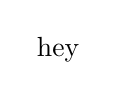
\begin{tikzpicture}
        \node at (0, 0) {hey};
    \end{tikzpicture}
    \caption{Illustration of the generative model of the LMM}
    \label{fig:generative_model_lmm}
\end{figure}

\section{The Linear Mixing Model}
\label{sec:lmm}

The Linear Mixing Model is given by the following generative model:
\begin{align} \label{eq:lmm}
    y(\vardot)\cond f(\vardot) &\sim \GP(f(\vardot), \Lambda), &
    f(\vardot)\cond H, x &= Hx(\vardot), &
    x &\sim \GP(0, K(\vardot, \vardot)) \tag{LMM}
\end{align}
where $\Lambda=\diag(\sigma_1^2,\ldots,\sigma_p^2)$ is a $p\times p$ diagonal multi-output kernel, $H$ a $p \times m$ matrix, and $K(\vardot,\vardot)$ an $m \times m$ diagonal multi-output kernel, where $K(t, t) := I$.
Intuitively, the data $y$ is generated by projecting $x$, which takes values in $\R^m$, into the higher dimensional space $\R^p$ via the linear map $H$, and finally adding noise.
This means that the data lives around the $m$-dimensional subspace that is the columns space of $H$.
The generative process is illustrated in blah and bleh.
Two main restrictions: correlations between the outputs are fixed in time, and no delays.
We call $x$ the \textit{latent processes}: motivation.

Connection with other models.

Discuss data lies on a lower dimensional subspace. Should be able to summarise.

\begin{proposition} \label{prop:augmentation}
    Augment the LMM by another process $u$:
    \begin{align*}
        u(\vardot)\cond x(\vardot) \sim \GP(x(\vardot), (H^\T \Lambda^{-1} H)^{-1}).
    \end{align*}
    Then $p(f\cond y) = p(f\cond u=Ty)$ where $T=(H^\T \Lambda^{-1} H)^{-1} H^\T \Lambda^{-1}$.
\end{proposition}

Elaborate on proposition.

\section{The Orthogonal Linear Mixing Model}
\label{sec:olmm}

Equation \eqref{eq:lmm} models a multi-output time-series problem as a vector projected into a fixed basis set defined by the columns of the mixing matrix, $H$, with time-varying coefficients given by the latent processes (modelled independently as GPs). The traditional LMM imposes no constraints over $H$, reflecting the usual freedom of basis choice. 
However, it is often very convenient to choose to work with an orthogonal basis set, as that provides a very simple way of computing the coordinates of a given vector and simplifies some expressions due to vanishing terms. With that in mind, one can opt to decompose $H$ via an SVD into three terms, $U$, $S$ and $V$, with $S$ diagonal and $U$ and $V$ orthogonal (i.e., $U U^\T = I$). 
By incorporating $V$ into the kernel matrix, i.e.\ by incorporating a rotation into the original latent processes, it is possible to write a new mixing matrix, $H_o$, that defines an orthogonal (but not necessarily orthonormal) base. That is:

\begin{equation}
    \mathbf{y(t)} = H \mathcal{GP}(0, K) = U S V \mathcal{GP}(0, K) = U S^{1/2} \mathcal{GP}(0, S^{1/2}V K V^\T S^{1/2}) = H_o \mathcal{GP}(0, K_o).
    \label{ortH}
\end{equation}
\todo{The GP notation requires some explanation}

Thus, \cref{ortH} shows that any LMM can be expressed in terms of an orthogonal basis set. 
That, however, makes it such that now the time-varying coefficients are given by a new GP, defined by a new kernel, $K_o$. 
For a given time stamp, $t_0$, since the original kernel matrix $K$ is such that the latent processes are independent and normalised, we have that $K_o(t_0, t_0) = S^{1/2}V V^\T S^{1/2} = S$ thus there are no instantaneous correlations between different latent processes. 
Interestingly enough, when we consider the correlations between two distinct time stamps, $t_0$ and $t_1$, $K(t_1, t_0) \neq I$ thus $K_o(t_1, t_0)$ may not be diagonal, meaning that different latent processes are now correlated in a non-instantaneous way, i.e., while $x_i(t_0)$ and $x_j(t_0)$ are uncorrelated, $x_i(t_0)$ and $x_j(t_1)$ may present correlation. 
Observing that this kind of behaviour is unusual and not necessarily desirable, we can choose to constrain $H$ such that $S^{1/2}V = I$ and $H = US^{1/2}$, in such a way that our basis set is orthogonal and all latent processes are completely independent, both instantaneously and non-instantaneously. 
This is the heart of the OLMM and leads to \cref{prop:independent_prediction}. \todo{Need to be much clearer about the $\sigma^2 I$ noise assumption. It's crucial, and it would be misleading not to highlight it.}

\begin{proposition} \label{prop:independent_prediction}
    Suppose that $H=US^{\frac{1}{2}}$ where $U$ is orthogonal and $S^{\frac{1}{2}}$ is diagonal, and that $\Lambda = \sigma^2 I + H D H^\T$ where $\sigma^2$ is the observation noise and $D$ is the diagonal matrix of the latent process noises.
    Augment the LMM by another process $u$:
    \begin{align*}
        u(\vardot)\cond x(\vardot) \sim \GP(x(\vardot), \sigma^2 S^{-1} + D).
    \end{align*}
    Then $p(f\cond y) = p(f\cond u = T y)$ where $T=S^{-\frac{1}{2}} U^\T$.
\end{proposition}

Note that this choice for $H$ is without loss of generality for $\E(y y^\T)$;
in other words, we do not restrict the spatial correlation in any way.

In a similar way that much of the power of the LMM comes from allowing us to easily exploit the low rank structure of covariances, the OLMM adds to that by allowing us to explore the independence of the latent processes. 
The real power of this approach becomes apparent when we look at the probability density function. As stated by \cref{prop:independent_learning}, it decouples the expression into separate contributions from each latent process, effectively reducing the complexity of the learning process from $\O(n^3m^3)$ to $\O(n^3m)$ and painting the perfect scenario for parallelising computations.

\begin{proposition} \label{prop:independent_learning}
    Assume the conditions from \cref{prop:independent_prediction}.
    Let $Y$ be observations for $y$ stacked into a $p \times n$ matrix.
    Then, letting $T_i = S_{ii}^{-\frac{1}{2}}U_{:,i}^\T$,
    \begin{align*}
        p(Y)
        &= \Normal(\operatorname{vec} Y;0,\sigma^2 I_{pn}) \prod_{i=1}^m
        \frac
            {\Normal(T_i Y ; 0, K_i + (\sigma^2/S_{ii} + D_{ii}) I_n)}
            {\Normal(T_i Y ;0, \sigma^2/S_{ii}I_n)}. \qedhere
    \end{align*}
\end{proposition}

In practice, computing the expression defined by \cref{prop:independent_learning} is remarkably simple. 
The first term represents the noise contributions and decouples each time stamp, leading to $n$ single-output GP computations. The product term is computed by projecting the observations $Y$ into the $ith$ latent process, via $Y \xrightarrow{} S^{-1/2}YU_{i,:}$, and doing two single-output GP computations (for each of the $m$ latent processes).

The OLMM, thus, reduces a multi-output GP problem to a projection followed by several simple single-output GP problems. 
Moreover, any technique that is applicable to single-output GP problems, such as inducing points \cite{Titsias:2009:Variational_Learning, Bui:2016:A_Unifying_Framework_for_Gaussian}, can be immediately leveraged by the OLMM. 

\section{Preliminary Experiments}
\label{sec:experiments}

We perform three sets of experiments with different goals. 
In the first experiment, we apply both the LMM and the OLMM to randomly generated data and analyse their speed and memory performance as a function of the number of latent processes. 
In the second experiment, we generate synthetic data from an LMM prior (with a non-orthogonal mixing matrix) and study how closely an OLMM model can reproduce that. 
Lastly, we apply the OLMM to a very large real-world data set, which is beyond the reach of the LMM, and compare its performance with that of individual GPs.

\subsection{Scaling experiments}
\label{subsec:scaling}

In this experiment, we generated a random matrix with 1500 observations for 20 different outputs as the input data.
Both the LMM and the OLMM models were constructed by using a mixing matrix of the form $H = U S^{1/2}$, with $U$ orthogonal and $S^{1/2}$ diagonal, squared exponential kernels for every latent process and zero mean.
We then proceeded to time and measure the memory requirement for a single computation of the log-likelihood of the data as a function of the number of latent processes.
The implementation of the LMM we adopted leverages the matrix lemma in order to scale with the number of latent processes, instead of with the number of outputs.
\cref{fig:tscale} shows that, as previously stated, the LMM scales in time as $\O(n^3m^3)$, while the OLMM scales as $\O(n^3m)$. 
In our case, this translates into either taking a couple of seconds for the OLMM or taking over 10 minutes for the LMM, using 25 latent processes.

\begin{figure}
    \centering
    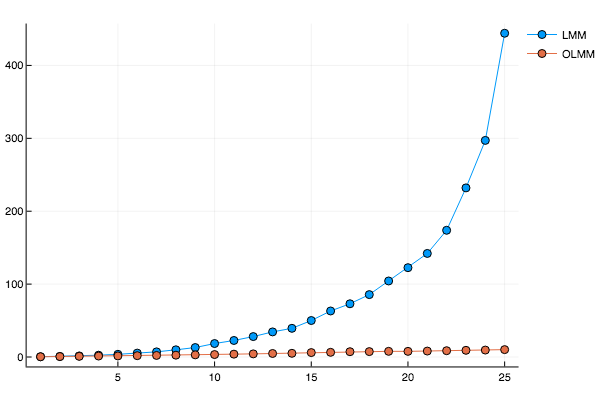
\includegraphics[width=8cm]{timescaling.png}
    \caption{SHITTY PLACEHOLDER FIGURE, REPLACE!!!! Time scaling of a single computation of the data log-likelihood for the LMM and for the OLMM as a function of the number of latent processes.}
    \label{fig:tscale}
\end{figure}

Although not as striking as the one presented on time, the OLMM also brings significant memory gains over the LMM, as shown in \cref{fig:mscale}. 
While memory scales as $\O(n^2 m^2)$ \todo{Check this, there is a different statement in the introduction} for the LMM, it scales as $\O(n^2 m)$ for the OLMM.
In our case, this means utilising less than 5GB of memory for the OLMM, as opposed to about 45GB for the LMM, again, using 25 latent processes. 
Note that this is a measure of total allocations, not of instantaneous RAM memory usage.

\begin{figure}
    \centering
    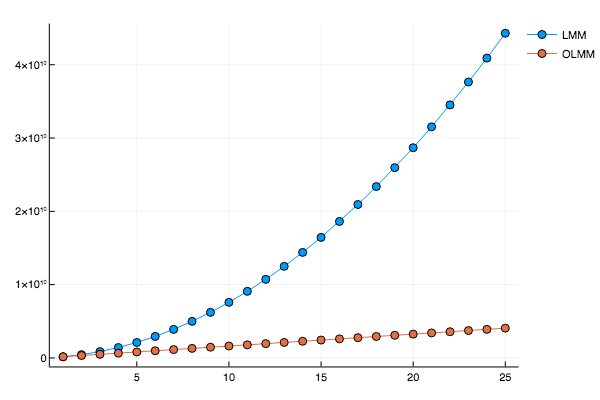
\includegraphics[width=8cm]{memscaling.png}
    \caption{SHITTY PLACEHOLDER FIGURE, REPLACE!!!! Memory scaling of a single computation of the data log marginal likelihood for the LMM and for the OLMM as a function of the number of latent processes. \textcolor{red}{we probably want to put these figures side by side to save space}}
    \label{fig:mscale}
\end{figure}

Thus, we show that, even for reasonably small systems, the OLMM greatly outperforms the LMM in both speed and memory.

\subsection{Reconstruction experiments}

Besides speed and memory performance, it is also paramount to assess accuracy.
To that end, we perform the following experiment: an LMM prior is created, with a mixing matrix that \emph{cannot} be written as $H = U S^{1/2}$, with 3 latent processes and with 6 outputs.
Kernels are squared exponentials with randomly chosen length-scales, variances and, in some cases, periodicities.
We, then, build three other models: an OLMM initialised with a mixing matrix defined by $H_o = U S^{1/2}$ with $U, S, V = svd(H)$, $H$ the prior mixing matrix; an OLMM initialised with a random matrix; and an LMM initialised with a random matrix. All models share the same number of latent processes and the same latent kernels with the prior.
For all three models, the mixing matrix was trained via the Adam algorithm for XXXXXXXX steps.
All calculations were performed using the stheno \cref{stheno} code.
The goal of these experiments is simply to see if the extra constraint over the mixing matrix increases the difficulty in the learning process.

blablabla

\paragraph{Scaling of the OLMM.}


\paragraph{Orthogonality Constraint.}
\begin{itemize}
    \item Pick output and latent dimensionalities for LMM + number of data to observe. Choose prior over all parameters. (Eric)
    \item Sample eg. 1000 times from the LMM prior. (Eric)
    \item Assess performance (ie. NLML) of LMM given exact parameters. (Eric)
    \item Assess performance (ie. NLML learning curves) of LMM with learned parameters using the correct latent dimensionality. (Eric)
    \item Assess performance (ie. NLML learning curves) of OLMM with learned parameters for a variety of latent dimensionalities. (Will)
    \item Questions this addresses:
    \begin{itemize}
        \item How does OLMM compare with true model?
        \item Given that we probably can't recover the true model in practice, how does the OLMM compare with the LMM that we can actually learn?
        \item If the latent dimensionality of the OLMM needs to increase to compensate for the orthogonality constraints on the mixing matrix, by how much do we generally need to increase it?
        \item If we increase the dimensionality, and hence the number of model parameters, presumably our data efficiency decreases (ie. kless favourable learning curve). If so, by enough that we care?
    \end{itemize}
\end{itemize}

\paragraph{Climate Modelling.} This experiment is more for show than anything else. Just compare OLMM with independent GPs. We need to sort out some memory-related issues here. (Will)

\begin{itemize}
    \item CMIP5 General Circulation Model data over Europe
    \item $n=500$ points used to learn parameters, $n=1000$ points used to test
    \item $m=100$ latent processes used for OLMM.
    \item Goal is to de-noise the simulator
    \item Compared with reanalysis temperature data
    \item The point is in no way the specifics of the problem, but rather that we've been able to run a large multi-output GP on a problem and use exact inference.
\end{itemize}

\section{Conclusion}
\label{sec:conclusion}

In this paper we presented the Orthogonal Linear Mixing Model, OLMM, which models a multi-output time series problem via an orthogonal basis with time-varying coefficients given by independent GPs and represents a variation over the traditional Linear Mixing Model, LMM.
Under such framework, latent processes decouple and the problem is reduced to a set of single-output GP problems.
Despite the LMM being one of the most popular multi-output GP models, due to its simplicity and ability to model reasonably large systems, we show that the OLMM significantly outperforms it, both in speed and in memory. 
Moreover, all techniques that are applicable to single-output GPs can be extended to the OLMM.
Effectively, the OLMM is a cheap, tractable, interpretable and accurate model for large multi-output time series.

We show the power of the model via three experiments. 
First, we show the significant speed and memory gains that the OLMM present over the LMM, which can easily reach orders of magnitude, even for relatively small systems.
Second, we show that the extra constraint over the mixing matrix does not significantly increase the difficulty in the learning process, with an OLMM model performing very closely to an LMM prior, whose mixing matrix was intentionally built such as not to satisfy the conditions for the OLMM.
Lastly, we apply the model to a notably large and challenging real-world data set and...

Moreover, we also cure cancer and solve the Israel-Palestine conflict.

\clearpage
\bibliographystyle{unsrtnat}
\bibliography{bibliography}

\end{document}